%----------------------------------------------------------------------------
\chapter{4lang}
\label{chap:4lang}
%---
The 4lang system is in the main focus of our work, in this chapter we will discuss the formalism and possible applications. 4lang also means the manually built dictionary of mapping more than 2000 words to graphs, this dictionary is described in \cite{Kornai:2013}. After discussing the main formalism of 4lang, we will demonstrate our baseline for the machine comprehension task.

\section{The formalism}
The \texttt{4lang} system of semantic representation \cite{Kornai:2015a}
represents the meaning of linguistic units (both words and phrases)
as directed graphs of syntax-independent concepts. Every node of a 4lang graph is a concept, which means that they are not taken as words, and they don't have any grammatical functions, like part-of-speech, voice, tense, etc.\cite{Recski:2016}.
Since these concepts have no grammatical attributes and no event structure, e.g.
the phrases \textit{water freezes} and \textit{frozen water} would both be
represented as \textit{water}~$\xrightarrow0$~\textit{freeze}. This also means that 4lang defines a many-to-one relation between the words and concepts. 

\textbf{4lang} formalism defines three types of edges:
\begin{itemize}
	\item \textbf{The 0-edge} represent represent attribution (\texttt{dog
		$\xrightarrow0$ large}), hypernymy (\texttt{dog $\xrightarrow0$ mammal}) and unary predication (\texttt{dog  $\xrightarrow0$ bark})
	\item \textbf{1- and 2-edges} those representing binary relations are connected to their arguments
	via edges labeled \texttt{1} and \texttt{2}, e.g \texttt{cat $\xleftarrow1$ catch $\xrightarrow2$ mouse}. Binaries that are shown with uppercase are binaries that must have two outgoing edges as shown in Figure \ref{fig:4langbin}. If we look at the sentence \textit{"Kinga broke Adam's bike"}, and the corresponding graph shown in Figure \ref{fig:4langbin}, if the 0-connection wouldn't be present between \textit{Kinga} $\xrightarrow0$ break, that would mean we consider that the relationship depend on whether the object of breaking is established or not. So in \textbf{4lang} the connection of 0-edge is present between a subject and a predicate regardless of the other arguments.
\end{itemize}

\begin{figure*}[h]
	\centering
	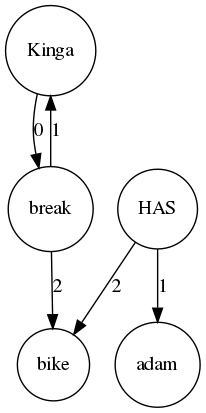
\includegraphics[height=0.5\textwidth]{figures/binary4lang}
	\caption{4lang with binaries}
	\label{fig:4langbin}
\end{figure*}

The example in
Figure~\ref{fig:bird} shows the \texttt{4lang} definition of the
concept \texttt{bird}. This definition was built manually, as part of
the \texttt{4lang} dictionary \cite{Kornai:2013}, but similar
definitions have been created automatically from definitions of
monolingual dictionaries such as Longman, using the
\texttt{dict\_to\_4lang} tool \cite{Recski:2016d}.

The open-source 4lang pipeline\footnote{\url{https://github.com/kornai/4lang}}
contains tools for generating
directed graphs from raw text by mapping dependency edges in the output of the
Stanford parser \cite{deMarneffe:2006} to \texttt{4lang} subgraphs over
concepts corresponding to each word of the original sentence. The Standford parser builds a dependency tree from the raw text that captures the syntactical relations between the linguistics units. 4lang graph construction involves mapping from these relations to 4lang semantics graphs, assigning the dependencies to 4lang subgraphs. The mapping is presented in Table \ref{table:mapping}, and an example is shown for sentence \textit{"I like swimming"} in Figure \ref{fig:swimmingdep}, where we can see the dependency tree coming out of the Standford parser, and the corresponding 4lang graph is present in Figure \ref{fig:swimming}, where the mapping from the dependency tree to \textbf{4lang} graph is done. 

\begin{table}
	\centering
	%\small
	\begin{tabular}{lc}
		\toprule
		Dependency & Edge \\
		\midrule
		amod & \multirow{7}{*}{\edge{$w_1$}{0}{$w_2$}} \\
		advmod & \\
		npadvmod & \\
		acomp & \\
		dep & \\
		num & \\
		prt & \\
		\midrule
		nsubj & \multirow{4}{*}{\twoedges{$w_1$}{1}{0}{$w_2$}} \\
		csubj & \\
		xsubj & \\
		agent & \\
		\midrule
		dobj & \multirow{6}{*}{\edge{$w_1$}{2}{$w_2$}} \\
		pobj & \\
		nsubjpass & \\
		csubjpass & \\
		pcomp & \\ 
		xcomp & \\
		\midrule
		appos & \twoedges{$w_1$}{0}{0}{$w_2$} \\
		\midrule
		poss & \multirow{2}{*}{$w_2\xleftarrow1$ \texttt{HAS} $\xrightarrow2w_1$} \\
		prep\_of & \\
		\midrule
		tmod & $w_1\xleftarrow1$ \texttt{AT} $\xrightarrow2w_2$ \\
		\midrule
		prep\_with & $w_1\xleftarrow1$ \texttt{INSTRUMENT} $\xrightarrow2w_2$ \\
		\midrule
		prep\_without & $w_1\xleftarrow1$ \texttt{LACK} $\xrightarrow2w_2$ \\
		\midrule
		prep\_P & $w_1\xleftarrow1$ \texttt{P} $\xrightarrow2w_2$ \\
		\bottomrule
	\end{tabular}
	\caption{Mapping from Stanford dependency relations to 4lang subgraphs \cite[p. 12.]{Recski:2018}.}
	\label{table:mapping}
\end{table}

\begin{figure*}[h]
	\centering
	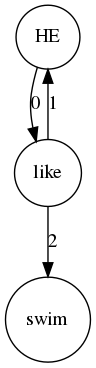
\includegraphics[height=0.5\textwidth]{figures/swimming}
	\caption{4lang example of a sentence}
	\label{fig:swimming}
\end{figure*}

\begin{figure*}[h]
	\centering
	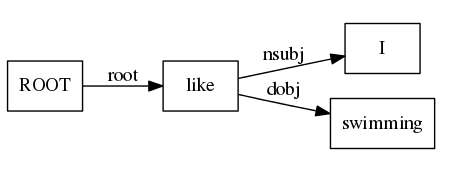
\includegraphics[width=0.5\textwidth]{figures/swimmingdep}
	\caption{Standford example of a sentence}
	\label{fig:swimmingdep}
\end{figure*}


\subsection{Expansion}
Optionally, the \texttt{4lang} system allows us to \textit{expand}
graphs, a process which unifies the graph with the definition graphs of
each concept. The implementation is written in the \textbf{dict\_to\_4lang} module, that extends the functionality of the discussed \textbf{text\_to\_4lang} pipeline with dictionaries. 4lang takes advantage of this, and implements the expansion step, which essentially is joining the definitions graphs to the main graph. This allow us to build a larger graph, that contains more information, and allow us to model the text better by simply adding the definition of words.

Let us look at the example sentence \textit{"My poor wife"}, that results the graph shown in Figure \ref{fig:mypoor}. If we are ready to make an assumption that taking word definitions into account results us a better model, and with this method we can have higher similarites between graphs whose sentences are also similar, than looking at the word poor definition is: \textit{having very little money and not many possessions}, we can build a definition graph and essentially join the two graphs together doing this for every word in the sentence resulting in a merged graph Figure \ref{fig:mypoorexpanded}. If we look at the graph, it is clear that the expanded graph gives us much more accurat context and definition. Our work was build around the expanded graph, and we will se that how better it actually performs on a real task. This will be the main topic of the next chapter.

\begin{figure}
	\centering
	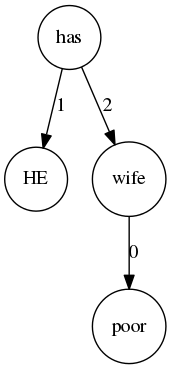
\includegraphics[scale=0.5]{figures/mypoor}
	\caption{4lang definition of sentence \textit{"My poor wife"}.}
	\label{fig:mypoor}
\end{figure}

\begin{figure}
	\centering
	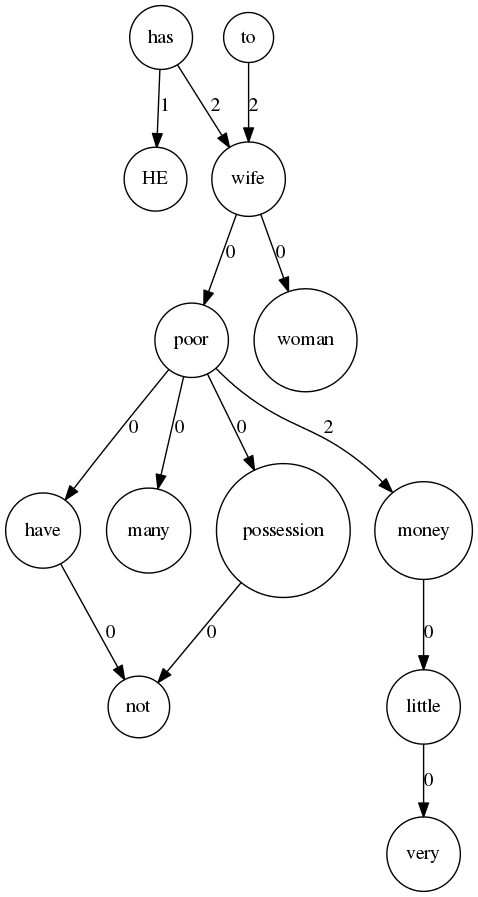
\includegraphics[scale=0.5]{figures/mypoorexpanded}
	\caption{4lang definition of expanded sentence \textit{"My poor wife"}.}
	\label{fig:mypoorexpanded}
\end{figure}

The beginning of our research we put a high emphasis on generating graphs from text with a highly automated method, so besides being an open-source software library,
the \texttt{4lang} we made the accessible via a public
REST API at \url{http://hlt.bme.hu/4lang}. We can generate graphs with raw text by calling the service. Currently our service have multiple endpoints, with each of them representing different methods.
If you interested in only processing a single sentence, you can call the following endpoints:

\begin{itemize}
	\item \textbf{/sendef} - Returns the graphs built from the sentence.
\item \textbf{/senexp} - Returns the graphs, where the word's definition has been added to the graph.
\item \textbf{/senabs} - Calling this function, we defined some rules, where we can build a more abstract graph using the definitions, this is more of a future work, I will talk about it  a bit in the last chapter.
\end{itemize}
You can get a word's definition by calling the defined endpoint:
\begin{itemize}
	\item \textbf{/definition} - Returns the graphs built from the word's definition.
\end{itemize}


\begin{figure}[!htb]
	\centering
	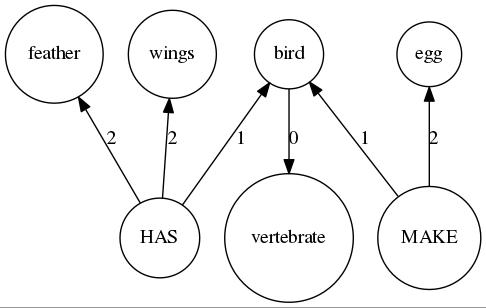
\includegraphics[scale=0.5]{figures/bird}
	\caption{4lang definition of \texttt{bird}.}
	\label{fig:bird}
\end{figure}

Graphs generated by the \texttt{4lang} parser have previously been used
successfully in measuring semantic similarity. The current state of the
art system on the \texttt{SimLex-999} benchmark \cite{Hill:2014a}
outperforms previous top systems by utilizing a simple similarity metric
between \texttt{4lang} definitions of pairs of English words
\cite{Recski:2016c}, this was the main idea of trying it in a different task with a different state-of-the-art system.

In the next chapter, I will briefly discuss the machine comprehension challenge, and I will introduce our baseline method for solving it. After that We will present how it is applicable to an already working system.